\documentclass[a4paper,12pt]{article}

%%% Работа с русским языком
\usepackage{cmap}					% поиск в PDF
\usepackage{mathtext} 				% русские буквы в формулах
\usepackage[T2A]{fontenc}			% кодировка
\usepackage[utf8]{inputenc}			% кодировка исходного текста
\usepackage[english,russian]{babel}	% локализация и переносы

%%% Дополнительная работа с математикой
\usepackage{amsfonts,amssymb,amsthm,mathtools} % AMS
\usepackage{amsmath}
\usepackage{icomma} % "Умная" запятая: $0,2$ --- число, $0, 2$ --- перечисление
\usepackage{varwidth,gensymb}
\usepackage{esvect} %вектор
%\usepackage{hyperref} %гиперссылки

%% Номера формул
%\mathtoolsset{showonlyrefs=true} % Показывать номера только у тех формул, на которые есть \eqref{} в тексте.

%% Шрифты
\usepackage{euscript}	 % Шрифт Евклид
\usepackage{mathrsfs} % Красивый матшрифт
\usepackage{indentfirst} % Красная строка после заголовка

%% Свои команды
\DeclareMathOperator{\sgn}{\mathop{sgn}}

%% Перенос знаков в формулах (по Львовскому)
\newcommand*{\hm}[1]{#1\nobreak\discretionary{}
{\hbox{$\mathsurround=0pt #1$}}{}}

%%% Работа с картинками
\usepackage{graphicx}  % Для вставки рисунков
\graphicspath{{images/}{images2/}}  % папки с картинками
\setlength\fboxsep{3pt} % Отступ рамки \fbox{} от рисунка
\setlength\fboxrule{1pt} % Толщина линий рамки \fbox{}
\usepackage{wrapfig} % Обтекание рисунков и таблиц текстом
\usepackage{caption}

%%% Работа с таблицами
\usepackage{array,tabularx,tabulary,booktabs} % Дополнительная работа с таблицами
\usepackage{longtable}  % Длинные таблицы
\usepackage{multirow} % Слияние строк в таблице
\usepackage{multicol}
% в преамбуле
\usepackage[left=2cm,right=2cm,
top=2cm,bottom=2cm,bindingoffset=0cm]{geometry}

%%% Заголовок

\title{Маятник Капицы с осциллирующим подвесом}
\date{\today}

\begin{document} % конец преамбулы, начало документа

\maketitle
\newpage

\section{Введение}
	Маятник Капицы - это система, состоящая из груза, прикреплённого к лёгкой нерастяжимой спице, которая крепится к вибрирующему подвесу. Особенностью маятника является устойчивость перевёрнутого (вертикального) положения маятника в случае быстрых вибраций подвеса. Ещё в 1908 году это явление наблюдал Эндрю Стефенсон, и только в 1951 году, когда П. Л. Капица экспериментально исследовал такой маятник, им была построена теория динамической стабилизации. Таким образом, Капица открыл новое направление в физике — вибрационную механику.

\section{Экспериментальные наблюдения}
	Исследуя данный маятник, мы можем получать разные колебания, в зависимости от характеристик движения подвеса, а именно частоты и амплитуды. Например, когда частота вынужденных осцилляций точки подвеса приблизительно вдвое больше частоты собственных колебаний маятника, нижнее положение равновесия становится неустойчивым: амплитуда первоначально сколь угодно малых колебаний маятника начинает прогрессивно нарастать со временем. Это явление называется параметрическим резонансом.
Другое ключевое свойство маятника - явление динамической стабилизации перевернутого положения. При достаточно больших значениях частоты и амплитуды осцилляций подвеса приведенный в перевернутое положение маятник не опрокидывается, и стремится к этому положению при умеренных отклонениях(устойчивое положение равновесия).

\section{Описание физической модели}
	Опишем физическую модель рассматриваемого маятника Капицы. Будем считать стержень длины $l$ невесомым, с массой $m$ на его свободном конце. За $a$ примем амплитуду колебательного движения подвеса, тогда закон движения подвеса записывается как 
\begin{equation}
\label{z(t)}
z(t) = a \cdot \cos{wt}
\end{equation}
Таким образом, в нашем случае $z(0) = a$.

	Перейдя в неинерциальную систему отсчета, связанную с подвесом, заметим, что на груз действует только две силы: сила тяжести $m\overrightarrow{g}$ вертикально вниз и сила инерции $\overrightarrow{F_и} = -m\ddot{\overrightarrow{z(t)}}$, направление и значение которой зависит от ускорения подвеса в данный момент. Из~(\ref{z(t)}) получим, что 
\begin{equation}
\label{Fi}
\overrightarrow{F_и(t)} = mw^2\overrightarrow{z(t)}
\end{equation}

\newpage
\section{Параметрический резонанс}
Рассмотрим поведение системы в случае частоты принудительных осцилляций подвеса вдвое большей частоты собственных колебаний маятника. Таким образом, при движении маятника от точки максимального отклонения к нижнему положению равновесия, сила инерции действует на него вниз и ускоряет движение груза$(рис.\;1,a)$. В момент прохождения нижней точки равновесия подвес проходит положение $z = 0(рис.\; 1,б)$, и далее сила инерции действует на груз вверх, тем самым увеличивая амплитуду колебаний$(рис.\; 1,в)$. Это явление называется параметрическим резонансом.

\begin{figure}[h!]
\begin{minipage}[h]{0.43\linewidth}
\center{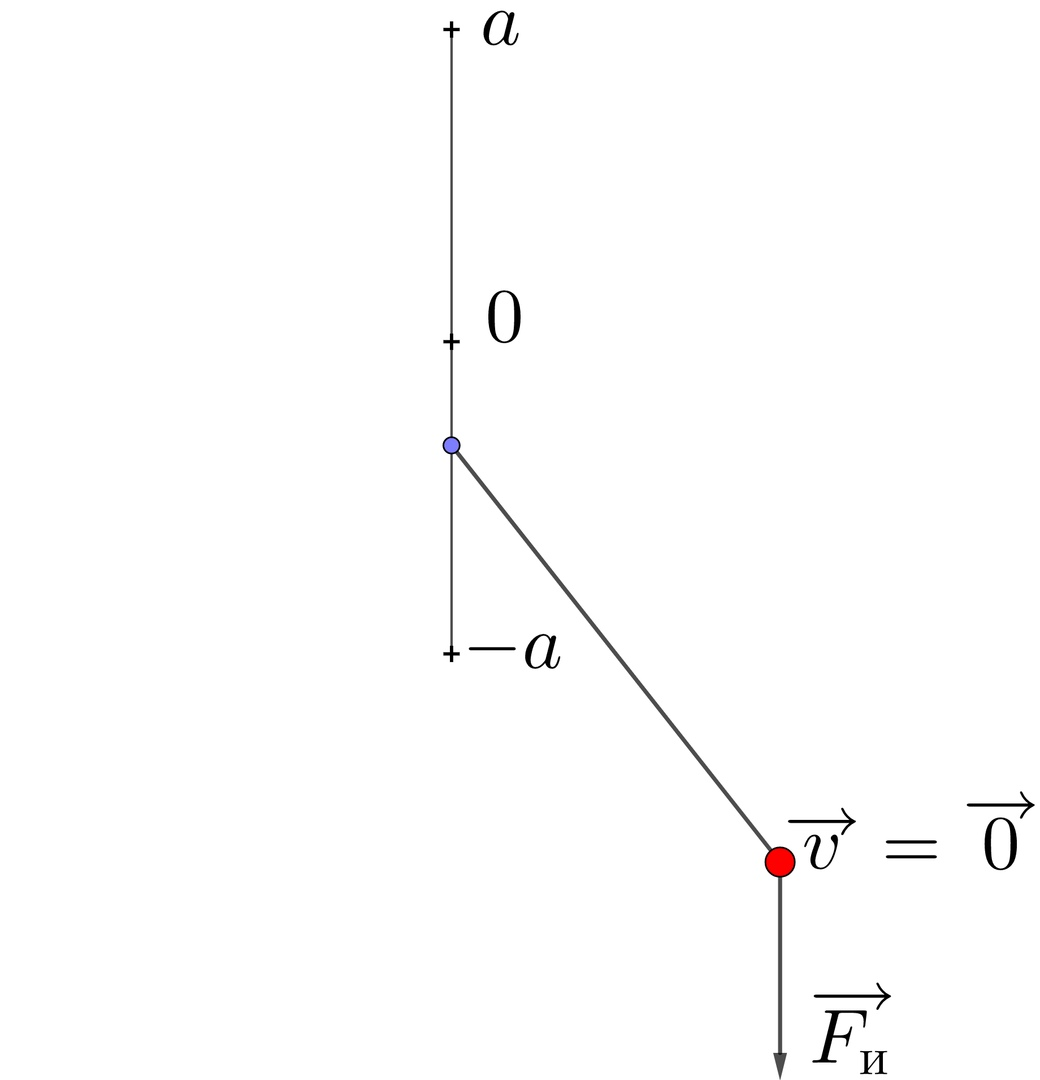
\includegraphics[width=\linewidth]{Pic1} \\ а)}
\end{minipage}
\hfill
\begin{minipage}[h]{0.43\linewidth}
\center{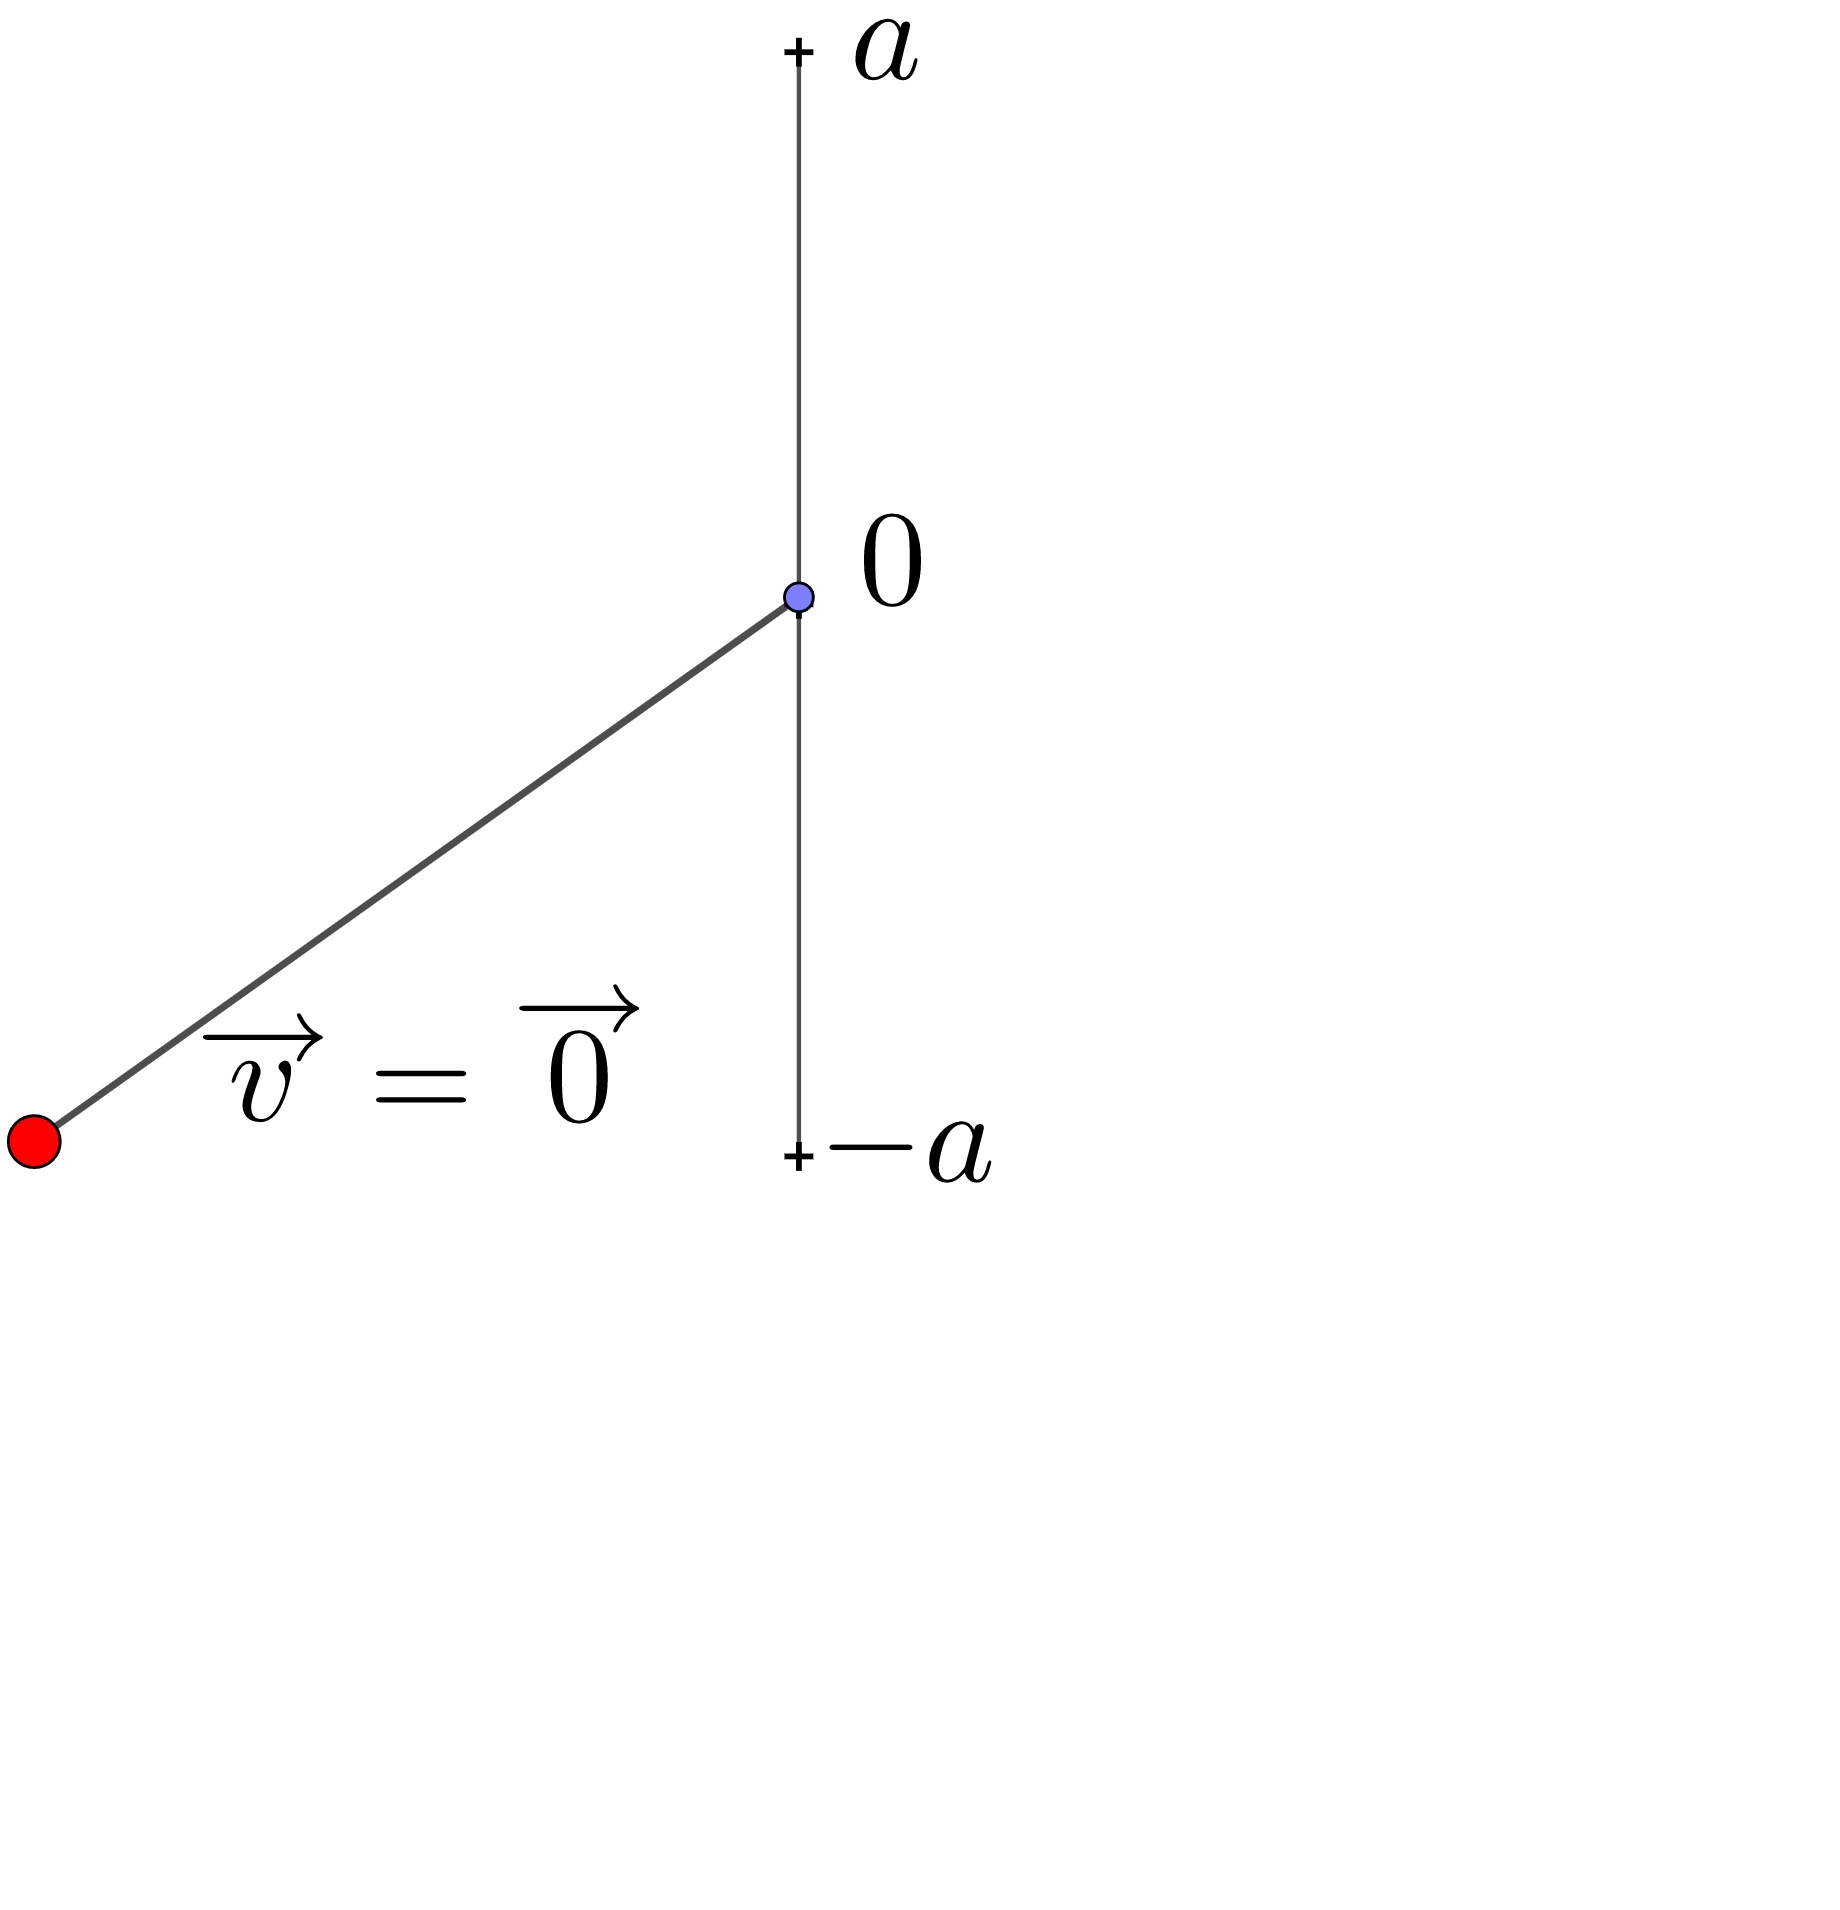
\includegraphics[width=\linewidth]{Pic2} \\ д)}
\end{minipage}
\begin{minipage}[h]{0.32\linewidth}
\center{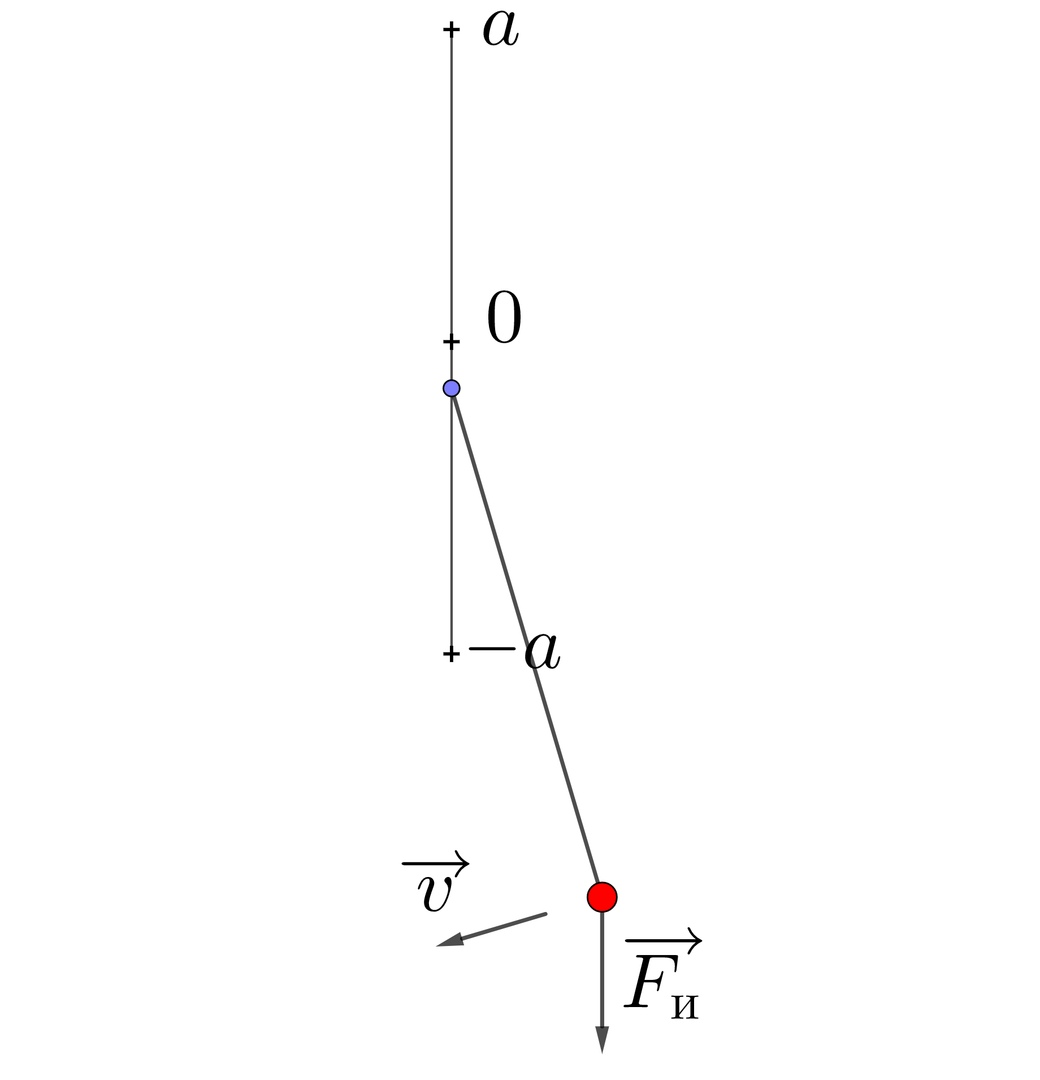
\includegraphics[width=\linewidth]{Pic3} \\ б)}
\end{minipage}
\begin{minipage}[h]{0.32\linewidth}
\center{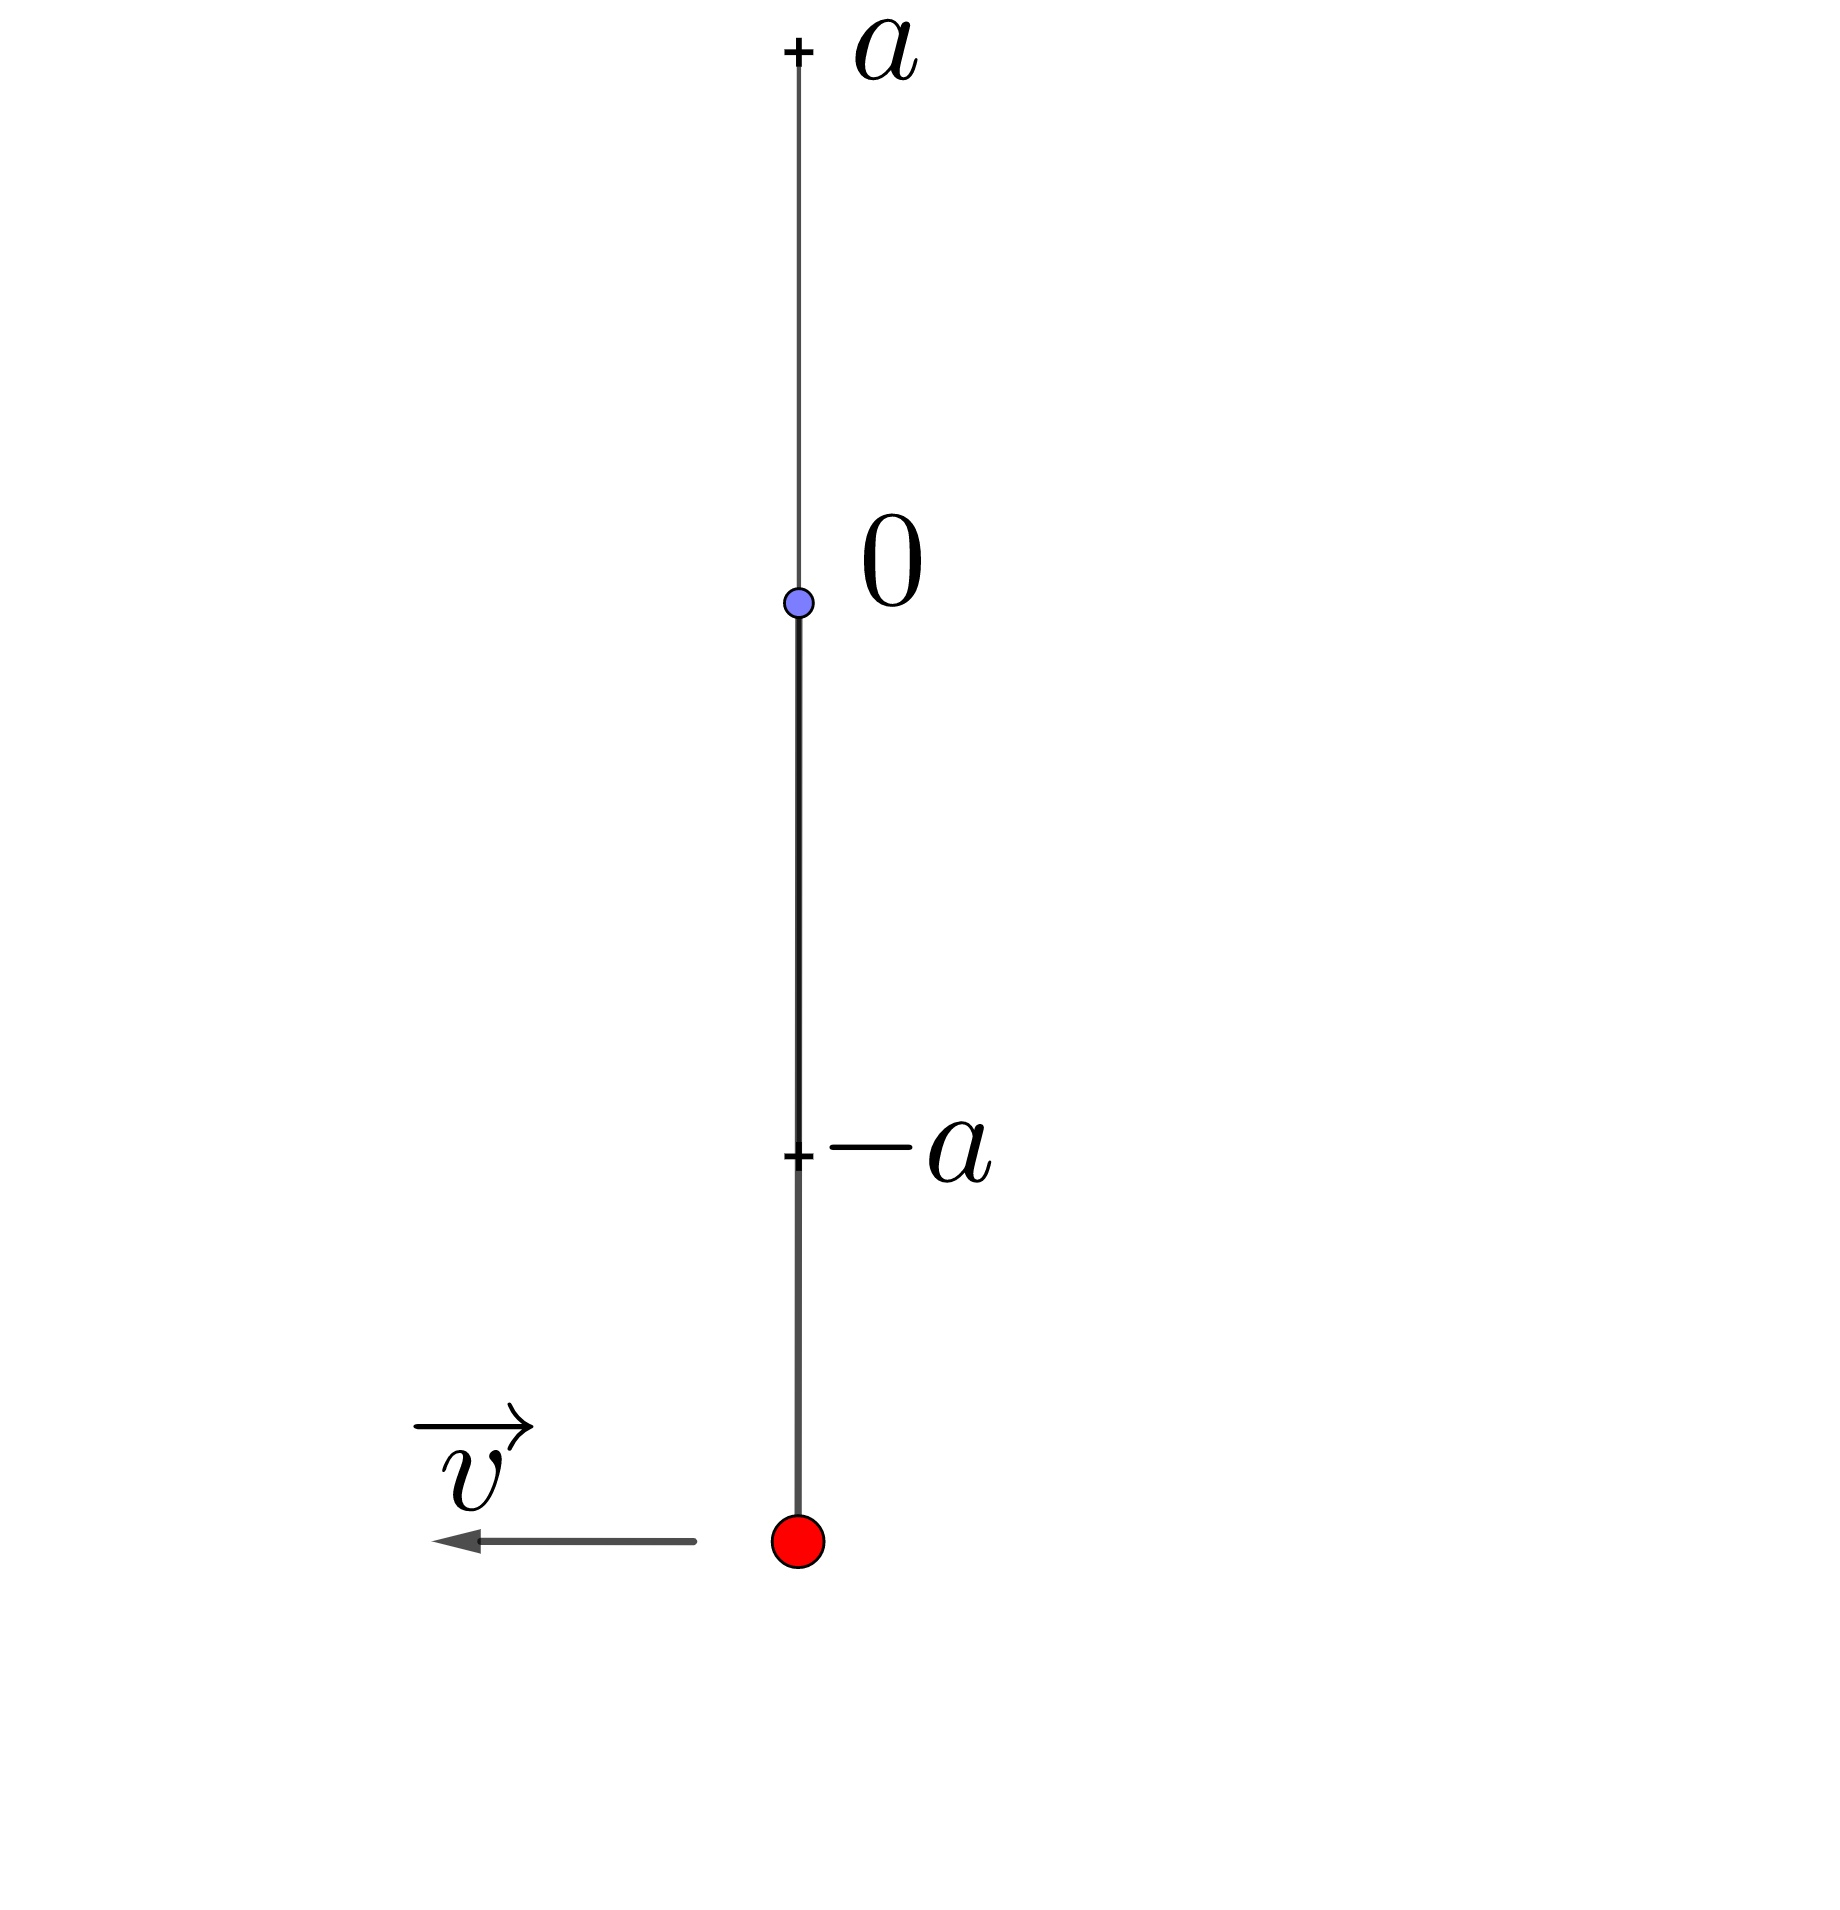
\includegraphics[width=\linewidth]{Pic4} \\ в)}
\end{minipage}
\begin{minipage}[h]{0.32\linewidth}
\center{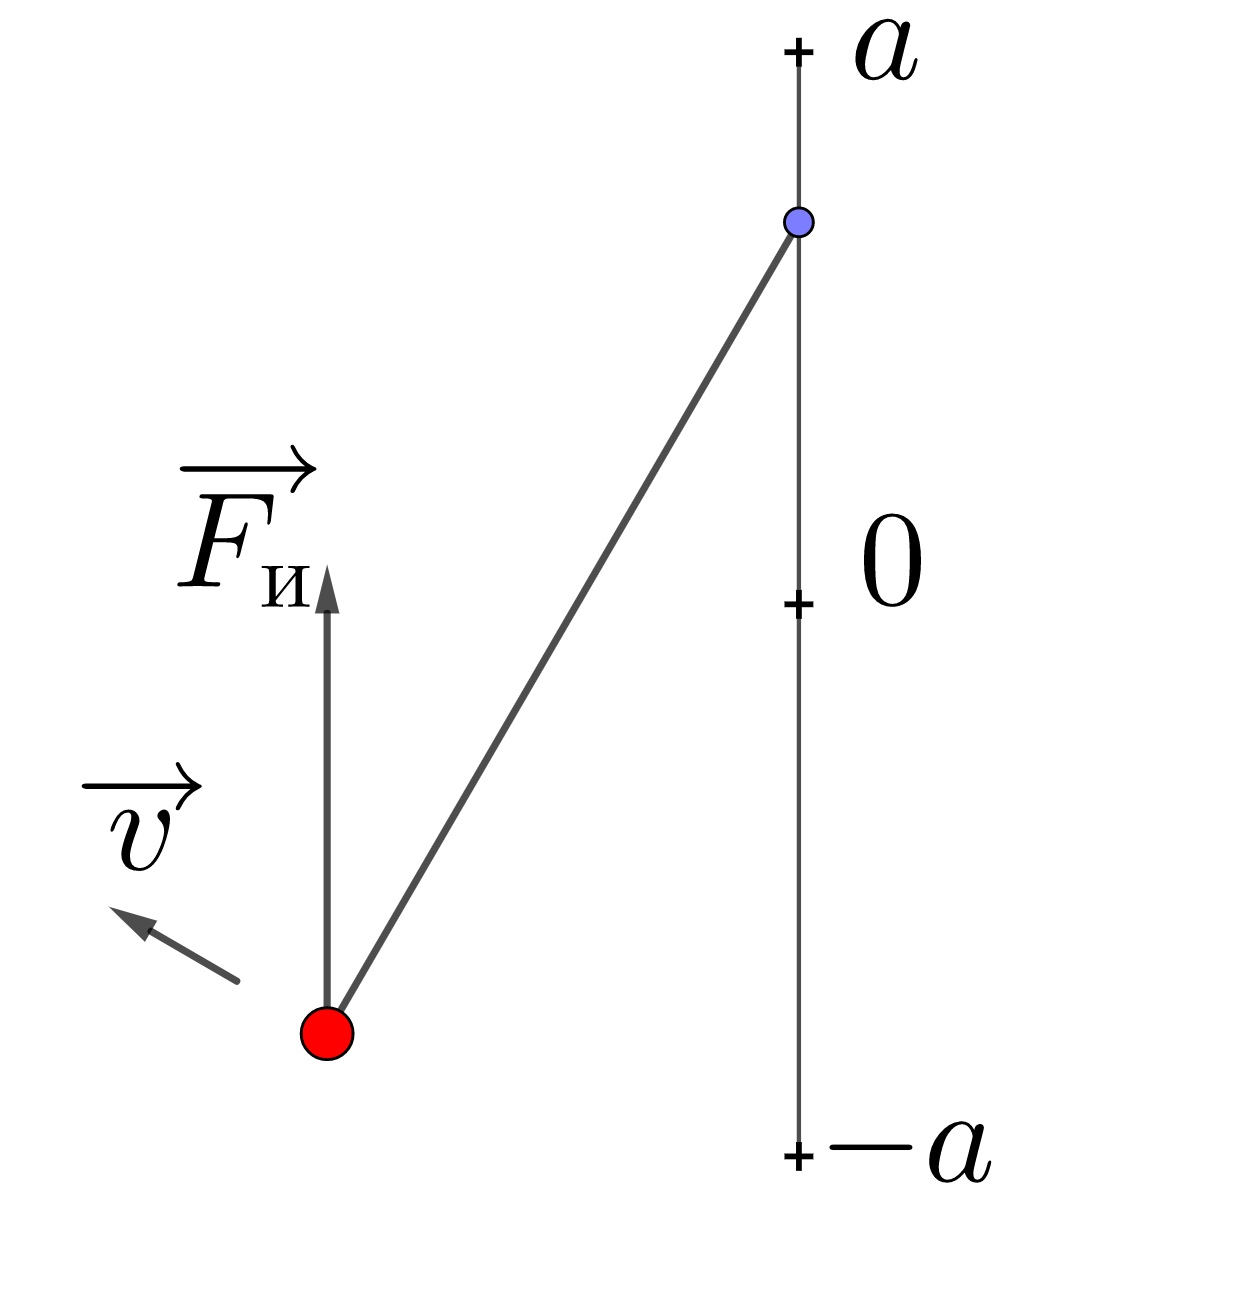
\includegraphics[width=\linewidth]{Pic5} \\ г)}
\end{minipage}
\begin{minipage}[h]{\linewidth}
\center{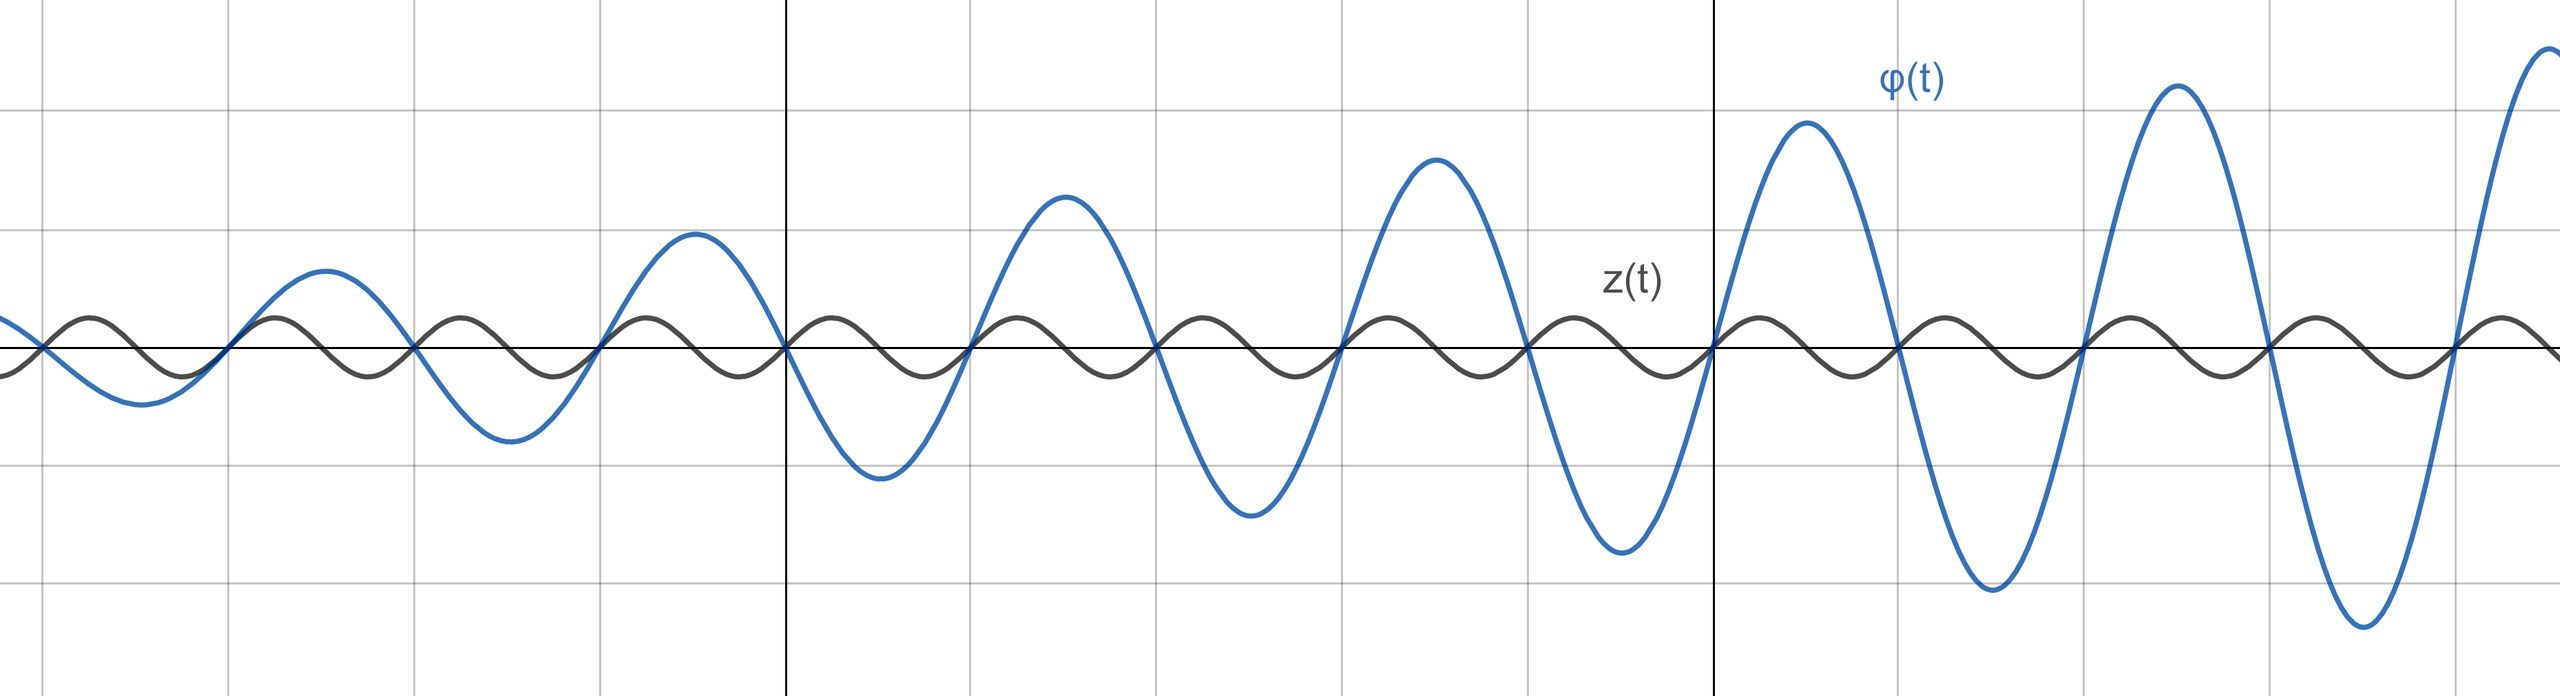
\includegraphics[width=\linewidth]{Pic6} \\ д}
\end{minipage}
\caption{Явление параметрического резонанса}
\label{im1}
\end{figure}

\section{Динамическая стабилизация перевернутого маятника}
\begin{wrapfigure}[18]{r}{6cm}
	\center{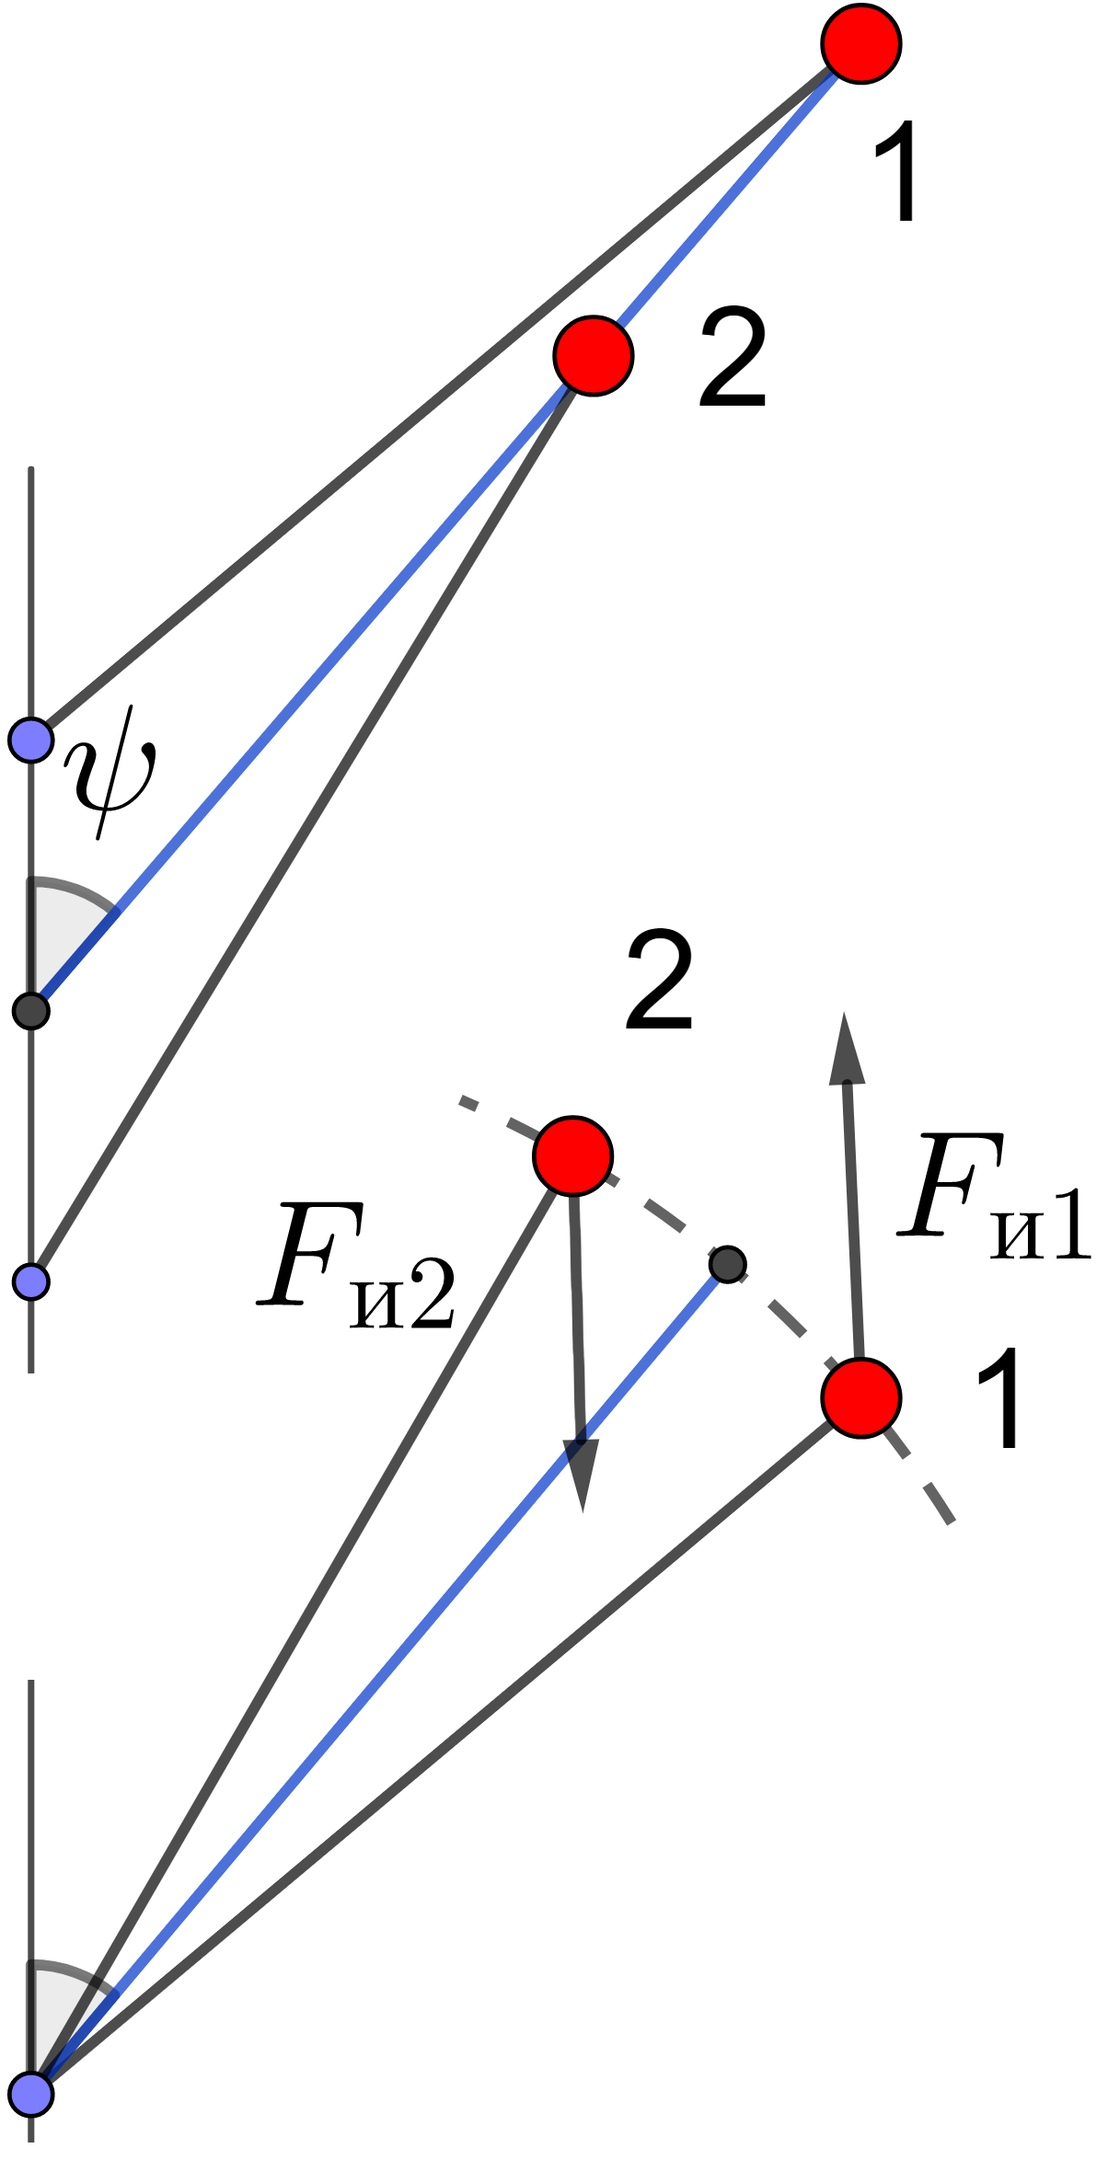
\includegraphics[width=0.6\linewidth]{Pic7}}\\
	\captionof{figure}{Маятник, отклоненный на угол $\psi$ от вертикали. Сверху в ЛСО, снизу - в СО подвеса}
\end{wrapfigure}
Рассмотрим маятник, отклоненный на некоторый угол $\psi$ от верхнего вертикального положения, и колеблющийся около новой позиции между точками$\;$ 1 и 2$(рис.\;2, a)$. В неинерциальной системе отсчета, связанной с подвесом, на груз в крайних положениях 1 и 2 действуют вертикальные силы тяжести и инерции, причем сила тяжести в обоих случаях направлена вниз, а сила инерции в точке 1 направлена вверх.\\

Так как плечо сил в положении 1 больше, то при достаточном значении силы инерции $F_{и1}$ момент сил, действующих на груз, в первом положении будет больше, причем это верно не только для крайних, но и для промежуточных пар положений грузов. Таким образом, средний момент сил, действующих на груз за время одного колебания подвеса положителен и возвращает маятник в вертикальное перевернутое положение при достаточной силе инерции.

\section{Количественное описание движения маятника}
Рассмотрим движение маятника при достаточно быстрых колебаниях подвеса(такие, частота которых много больше частоты собственных колебаний маятника $w_0 = \sqrt{l/g}$). В этом случае его можно рассмотреть как суперпозицию $"медленной"$ и $"быстрой"$ компонент движения. Углы отсчитываются от нижнего положения маятника против часовой стрелки. Таким образом, 
\begin{equation}
\varphi(t) = \psi(t) + \delta(t)
\label{angle}
\end{equation}
Здесь $\varphi(t)$ - угол отклонения маятника от нижнего положения, $\psi(t)$ - $"медленная"$ компонента, описывающая движение маятника, усредненное за период одного колебания подвеса, а $\delta(t)$ - $"быстрая"$, происходящая с частотой $w$ вынужденных колебаний подвеса. Геометрически, подставив $z(t)$ из~(\ref{z(t)}) получаем 
\[\delta(t) = -\dfrac{a\sin{\psi}\cos{wt}}{l}\]
Поскольку осцилляции подвеса приводят лишь к небольшим отклонениям $\varphi$ от $\psi$, то $\delta$ достаточно мал для приближения $\sin{\delta} \approx \delta, \cos{\delta} \approx 1$. Таким образом, 
\begin{equation}
\sin{\varphi} = \sin{\psi}\cos{\delta} + \sin{\delta}\cos{\psi} \approx \sin{\psi} + \delta\cos{\psi}
\end{equation}
Длина плеча силы тяжести и инерции равна $l\sin{\varphi}$. В течение одной осцилляции подвеса, $\psi$ можно считать постоянной, независящий от времени. Таким образом, средние значения момента сил тяжести и инерции равны соответственно
\begin{align}
\langle M_т \rangle &= \langle -mgl\sin{\varphi}\rangle = -mgl\langle\sin{\psi} + \delta\cos{\psi}\rangle = -mgl\sin{\psi}
\end{align}
\begin{equation}
\left.\begin{aligned}
\langle M_{F_и} \rangle &= \langle F_иl\sin{\varphi} \rangle = \langle mw^2al(\sin{\psi} + \delta\cos{\psi})\cos{wt} \rangle =\\&= mw^2al(\langle \sin{\psi}\cos{wt} \rangle + \langle \delta\cos{wt}\cos{\psi} \rangle) = mw^2al\cos{\psi}\langle-\dfrac{a}{l}\cos^2{wt}\sin{\psi}\rangle =\\&= -mw^2a^2\cos{\psi}\sin{\psi}\langle\dfrac{1}{2} - \dfrac{1}{2}\cos{2wt}\rangle = -\dfrac{1}{4}mw^2a^2\sin{2\psi}
\end{aligned}\right.
\end{equation}
Заметим, что $M_{Fи} > 0 \Leftrightarrow \sin{2\psi} < 0$, в этом случае 
\begin{equation}
\label{M}
\langle M \rangle = -mgl\sin{\psi} - \dfrac{1}{4}mw^2a^2\sin{2\psi} = -m\sin{\psi}(gl - \dfrac{1}{2}w^2a^2\cos{\psi})
\end{equation} 
При $\langle M \rangle > 0 \Leftrightarrow w^2a^2 > 2gl$ верхнее перевернутое положение маятника является устойчивым, и при небольших отклонениях маятник возвращается в это состояние. Подставив $w_0 = \sqrt{g/l}$ получим другой вид условия устойчивости перевернутого положения маятника
\begin{equation}
\label{ust}
\frac{a}{l}\cdot\frac{w}{w_0} > \sqrt{2}
\end{equation} 
Для оценки возможных отклонений можем приравнять $\langle M\rangle = 0$. Так мы получим критическое $\psi_{кр}$, при котором маятник уже не вернется в верхнее положение. Ближайшая такая точка к верхнему положению находится из равенства $\alpha_{max} = \pi - \psi_{кр}$, где $\cos{\psi_{кр}} = -\dfrac{2gl}{w^2a^2}$ $\Rightarrow \cos{\alpha_{max}} = -\cos{\psi_{кр}} = \dfrac{2gl}{a^2w^2} = 2\;(\dfrac{w_0l}{wa})^2$ 
Чем больше произведение $wa$ частоты и амплитуды осцилляций подвеса, тем ближе к $\pi/2$ максимально допустимое отклонение маятника $\alpha_{max}$ от перевернутого положения. Если отклонить маятник на угол, меньший $\alpha_{max}$, то он будет совершать сравнительно медленные колебания около перевернутого положения. Аналогичное поведение маятника наблюдается и при отклонении от нижнего положения равновесия. Но в этом случае частота медленных колебаний маятника больше, чем около перевернутого положения, т к частота увеличивается благодаря осицлляциям подвеса.
\newpage
\section{Энергия маятника}
Рассмотрим маятник в СО подвеса. Средний момент сил, действующий на груз, за одно колебание подвеса~(\ref{M}) создает изменение момента импульса $I\ddot{\psi}$, где $I = ml^2$.
\begin{equation}
\label{f2}
\ddot{\psi} = -\frac{g}{l}\sin{\psi} - \frac{1}{4}\frac{a^2}{l^2}w^2\sin{2\psi}
\end{equation}
Или, подставив $w_0^2 = g/l$:
\begin{equation}
\ddot{\psi} = -w_0^2\sin{\psi} - 	\frac{1}{4}\frac{a^2}{l^2}w^2\sin{2\psi}
\end{equation}
Движение маятника можно представить как движение частицы в эффективном потенциальном поле. Таком, что $M(\psi) = -dU(\psi)/d\psi$. Компоненты $U_{mg}$ и $U_и$ описывают действие сил тяжести и инерции соответственно. Таким образом, $U_{tot}(\psi) = U_{gr}(\psi) + U_{in}(\psi)$,
$U_{gr}(\psi) = mgl(1-\cos{\psi}), U_{in}(\psi) = \frac{1}{4}ma^2w^2(1-\cos{2\psi})$\\
\begin{wrapfigure}[12]{r}{7cm}
	\vspace{-7ex}
	\center{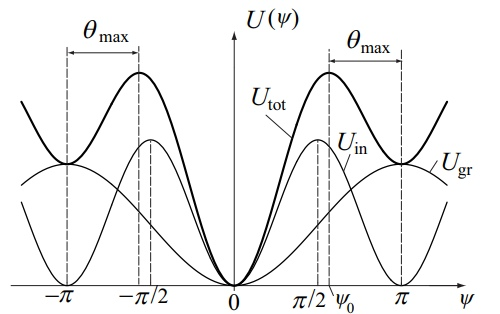
\includegraphics[width=1\linewidth]{Pic8}}\\
	\captionof{figure}{Графики потенциальных энергий}
\end{wrapfigure}
Графики показаны на рисунке 3, оба имеют синусоидальную форму, но период $U_{in}(\psi)$ вдвое меньше периода $U_{gr}(\psi)$. Их минимумы при $\psi = 0 $ совпадают, образуя абсолютный минимум полной функции $U_{tot}(\psi)$. Этот минимум соответствует нижнему устойчивому положению равновесия маятника. Соседний минимум $U_{in}(\psi)$ расположен при $\psi = \pi$, где $U_{gr}(\psi)$ имеет максимум, соотвествующий перевернутому маятнику.
Если выполняется критерий устойчивости перевернутого маятника~(\ref{ust}), то полный потенциал имеет дополнительные минимумы($\psi = \pm\pi$), соответствующие перевернутому маятнику. В точке $\psi = 0$ находится абсолютный минимум, соответствующий нижнему положению равновесия. Рассмотрим эти точки. При $\psi = 0$ $sin\psi = \psi$, при $\psi = \pi$ $sin\psi = sin(\pi - \theta) \approx \theta$, $cos\psi = -1$:
\begin{align}
w_{down}^2 &= \frac{a^2w^2}{2l^2} + w_0^2 & w_{up}^2 &= \frac{a^2w^2}{2l^2} - w_0^2
\end{align}

\end{document}	